\documentclass[12pt]{beamer}

\usepackage[english]{babel}
\usepackage[utf8]{inputenc}
\usepackage{tikz}

\usetheme{Copenhagen}
\setbeamertemplate{navigation symbols}{}

\title{The FLP Theorem}
\author[Jacopo Notarstefano]{
  Jacopo Notarstefano\\
  \texttt{jacopo.notarstefano [at] gmail.com}
}
\date{}

\begin{document}
  \begin{frame}[plain]
    \titlepage
  \end{frame}

  \begin{frame}{The Distributed Consensus Problem}
    \begin{definition}{}
    \end{definition}
  \end{frame}

  \begin{frame}{Consensus Protocol}
  \end{frame}

  \begin{frame}{Message System}
  \end{frame}

  \begin{frame}{Partial correctness}
    A configuration \(C\) has \textbf{decision value} \(v\) if some process \(p\) is in a decision state with \(y_p = v\).

    \vspace{0.25cm}

    \begin{definition}[Partial correctness]
      A consensus protocol is \textbf{partially correct} if:
      \begin{enumerate}
        \item No accessible configuration has more than one decision value.
        \item For each \(v\in \{0,1\}\), some accessible configuration has decision value \(v\).
      \end{enumerate}
    \end{definition}
  \end{frame}

  \begin{frame}{Total correctness in spite of one fault}
    A process \(p\) is \textbf{nonfaulty} in run if it takes infinitely many steps, otherwise it is \textbf{faulty}.

    \vspace{0.25cm}

    A run is \textbf{admissible} if at most one process is faulty and all messages sent to nonfaulty processes are eventually received.

    \vspace{0.25cm}

    A run is \textbf{deciding} if some process reaches a decision state.

    \vspace{0.25cm}

    \begin{definition}[Total correctness in spite of one fault]
      A consensus protocol \(P\) is \textbf{totaly correct in spite of one fault} if it is partially correct and every admissibile run is deciding.
    \end{definition}
  \end{frame}

  \begin{frame}{Main result}
    \begin{theorem}[Fischer, Lynch, Paterson 1985]
      No consensus protocol is totally correct in spite of one fault.
    \end{theorem}

    \vspace{0.25cm}

    A configuration is \textbf{bivalent} if the set of decision values of configurations reachable from it has \(2\) elements. It is instead \textbf{\(0\)-valent} or \textbf{\(1\)-valent} according to the corresponding value.

    \vspace{0.25cm}

    \begin{proof}[Proof (sketch)]
      Given an initial bivalent configuration, we construct an admissible run that at each stage results in another bivalent configuration.
    \end{proof}
  \end{frame}

  \begin{frame}{Lemma 1}
    \begin{lemma}
      Suppose that from some configuration \(C\), the schedules \(\sigma_1\), \(\sigma_2\) lead to configurations \(C_1\), \(C_2\) respectively. If the sets of processes taking steps in \(\sigma_1\) and \(\sigma_2\), respectively, are disjoint, then \(\sigma_2\) can be applied to \(C_1\) and \(\sigma_1\) can be applied to \(C_2\), and both lead to the same configuration \(C_3\).
    \end{lemma}

    \vspace{0.25cm}

    In other words: \textbf{schedules about disjoint processes commute}.
  \end{frame}

  \begin{frame}{Proof of Lemma 1}
    \begin{proof}[Proof (Lemma 1)]
      \begin{figure}
        \makebox[\textwidth][c]{
          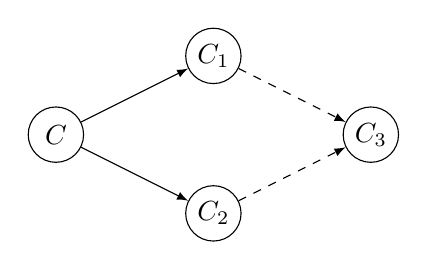
\begin{tikzpicture}
            \tikzstyle{configuration}=[draw,circle,inner sep=0pt,minimum size=20pt]

            \node (C) at (0,0) [configuration] {\(C\)};
            \node (C1) at (2,1) [configuration] {\(C_1\)};
            \node (C2) at (2,-1) [configuration] {\(C_2\)};
            \node (C3) at (4,0) [configuration] {\(C_3\)};

            \draw[-latex] (C) to (C1);
            \draw[-latex] (C) to (C2);
            \draw[-latex, dashed] (C1) to (C3);
            \draw[-latex, dashed] (C2) to (C3);
          \end{tikzpicture}
        }
      \end{figure}
    \end{proof}
  \end{frame}

  \begin{frame}{Lemma 2}
    \begin{lemma}
      \(P\) has a bivalent initial configuration.
    \end{lemma}

    \vspace{0.25cm}

    \begin{proof}[Proof (Lemma 2)]
    \end{proof}
  \end{frame}

  \begin{frame}{Lemma 3}
    \begin{lemma}
      Let \(C\) be a bivalent configuration of \(P\), and let \(e = (p,m)\) be an event that is applicable to \(C\). Let \(\mathcal{C}\) be the set of configurations reachable from \(C\) without applying \(e\), and let \(\mathcal{D} = e(\mathcal{C}) = \{ e(E) \vert E \in \mathcal{C} \text{ and } e \text{ is applicable to \(E\)} \}\). Then, \(\mathcal{D}\) contains a bivalent configuration.
    \end{lemma}

    \vspace{0.25cm}

    In other words: given a bivalent configuration and an event \(e\) applicable to it, \textbf{we construct another bivalent configuration having \(e\) as the last applied event}.
  \end{frame}

  \begin{frame}{Proof of Lemma 3}
    \begin{proof}[Proof (Lemma 3)]
    \end{proof}
  \end{frame}

  \begin{frame}{Proof of main result}
    \begin{proof}[Proof (main result)]
    \end{proof}
  \end{frame}
\end{document}
